\chapter{Implementierung}
\label{chap:implementierung}

\section{Technologische Basis}
Die Implementierung basiert auf einer sorgfältig ausgewählten technologischen Basis, die modernste Tools und Frameworks kombiniert, um eine effiziente, skalierbare und sichere Lösung zu gewährleisten. Die Haupttechnologien umfassen:

\begin{itemize}
    \item \textbf{Frontend:} Die Entwicklung des Frontends erfolgt mit React und TypeScript, um eine robuste und komponentenbasierte Architektur zu gewährleisten. Primereact wird als UI-Bibliothek eingesetzt, um eine konsistente Benutzeroberfläche zu realisieren und die Entwicklungszeit durch vorgefertigte, anpassbare Komponenten zu verkürzen. Vite dient als modernes Build-Tool, das durch schnelle Hot-Module-Replacement-Funktionen eine produktive Entwicklungsumgebung bietet.
    
    \item \textbf{Backend:} Das Backend basiert auf .NET Core und stellt RESTful APIs bereit, die eine zuverlässige und standardisierte Kommunikation ermöglichen. Middleware-Services wurden implementiert, um Aufgaben wie Authentifizierung, Fehlerbehandlung und Protokollierung zu übernehmen. Die Verwendung von Azure Active Directory (AAD) gewährleistet eine sichere Authentifizierung und rollenbasierte Zugriffskontrolle.
    
    \item \textbf{Azure Cloud:} Die Azure Cloud spielt eine zentrale Rolle bei der Implementierung, da sie Dienste wie Azure Service Bus zur asynchronen Kommunikation zwischen Systemkomponenten bereitstellt. Außerdem ermöglicht sie eine flexible und skalierbare Infrastruktur, die für die Anforderungen des Systems optimiert ist.
    
    \item \textbf{DevOps:} Zur Optimierung des Entwicklungs- und Bereitstellungsprozesses werden automatisierte CI/CD-Pipelines mit Azure Pipelines verwendet. Diese Pipelines integrieren automatisierte Tests, Builds und Deployments, um eine hohe Qualität und schnelle Iterationen sicherzustellen.
    
    \item \textbf{Versionskontrolle mit Git:} Git wurde als zentrales Versionskontrollsystem genutzt. Es ermöglicht effizientes Arbeiten mit Feature-Branches, Pull-Requests und das einfache Nachverfolgen von Änderungen. GitHub wurde als zentrale Plattform für die Zusammenarbeit und Code-Reviews verwendet.
    
    \item \textbf{SCRUM-Board:} Ein digitales SCRUM-Board wurde eingesetzt im DevOps, um Aufgaben zu planen, zu priorisieren und den Fortschritt in Sprints zu überwachen.

    \item \textbf{Testautomatisierung:} Tools wie Jest und React Testing Library wurden zur Sicherstellung der Codequalität eingesetzt. Automatisierte Tests wurden in die CI/CD-Pipeline integriert, um frühzeitig Fehler zu erkennen und zu beheben.

    \item \textbf{Containerisierung:} Docker wurde für die Bereitstellung einer konsistenten Entwicklungs- und Produktionsumgebung genutzt. Docker-Images für das Frontend und Backend werden in einer Azure Container Registry (ACR) gespeichert und ermöglichen schnelle und skalierbare Deployments.
    
    \item \textbf{Monitoring und Fehleranalyse:} Azure Application Insights wurde zur Überwachung von Systemmetriken wie Antwortzeiten, Fehlerraten und Benutzerinteraktionen integriert. Dies ermöglicht eine effiziente Fehlerdiagnose und Performance-Optimierung.
\end{itemize}

Diese technologische Basis bildet die Grundlage für die Implementierung einer modernen, leistungsfähigen Softwarelösung, die den Anforderungen an Skalierbarkeit, Sicherheit und Benutzerfreundlichkeit gerecht wird.

\section{Detailierte Architektur}
\subsection{Frontend-Architektur}
Das Frontend wurde mit einer komponentenbasierten Architektur entwickelt, die eine modulare und wiederverwendbare Struktur ermöglicht. Jedes UI-Element wurde als eigenständige Komponente konzipiert, um sowohl die Wartbarkeit als auch die Wiederverwendbarkeit zu maximieren. Diese Architektur fördert eine klare Trennung der Verantwortlichkeiten und ermöglicht eine einfache Anpassung und Erweiterung der Benutzeroberfläche.

Die Projektstruktur, wie in Abbildung~\ref{fig:frontend_code_paradigm} dargestellt, folgt bewährten Best Practices der modernen Frontend-Entwicklung. Der Ordner \texttt{components} enthält alle UI-Komponenten, während der Ordner \texttt{store} die State-Management-Logik beherbergt. Globale Konfigurationen werden im Ordner \texttt{config} verwaltet, während allgemeine Funktionen und Hilfsprogramme im Ordner \texttt{utils} zentralisiert sind. Der Aufbau fördert eine klare Trennung von Verantwortlichkeiten, was die Lesbarkeit und Wartbarkeit des Codes erheblich verbessert.

Ein weiteres zentrales Element ist das State-Management, das mithilfe von Redux Toolkit und Zustand realisiert wird. Diese Tools gewährleisten eine effiziente Verwaltung globaler und lokaler Zustände und ermöglichen es, komplexe Datenflüsse innerhalb der Anwendung zu steuern. Die Integration von Visualisierungsbibliotheken wie ApexCharts und React-ApexCharts trägt zur Erstellung interaktiver Diagramme wie Donut- und Radarcharts bei, die für die Darstellung und Analyse von Daten essenziell sind.

\begin{figure}[H]
    \centering
    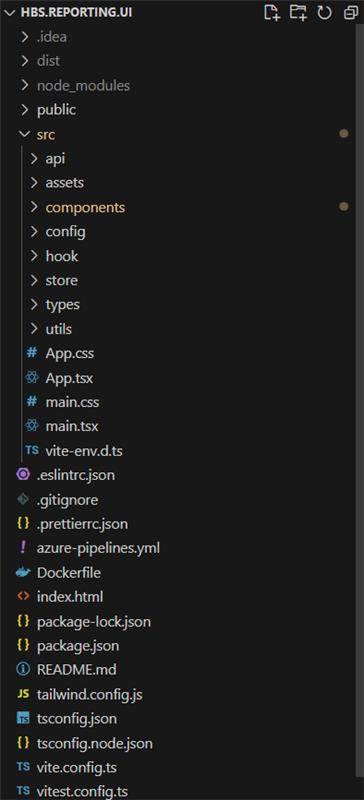
\includegraphics[width=0.4\textwidth, keepaspectratio]{images/frontendparadigma.jpg}
    \caption{Projektstruktur des Frontend-Paradigmas.}
    \label{fig:frontend_code_paradigm}
\end{figure}

In Abbildung~\ref{fig:frontend_code_paradigm} wird die Projektstruktur der Anwendung dargestellt. Die klare Trennung in Module wie \texttt{components}, \texttt{store} und \texttt{api} erleichtert nicht nur die Entwicklung, sondern fördert auch die Zusammenarbeit in Teams und die Skalierbarkeit des Systems. Diese Struktur bietet eine solide Grundlage für die Entwicklung moderner und leistungsstarker Webanwendungen.


\subsubsection*{Live Anwendung}
Die folgende Abbildungen zeigen die PROD Ausschnitte der Anwendung:

\begin{figure}[H]
    \centering
    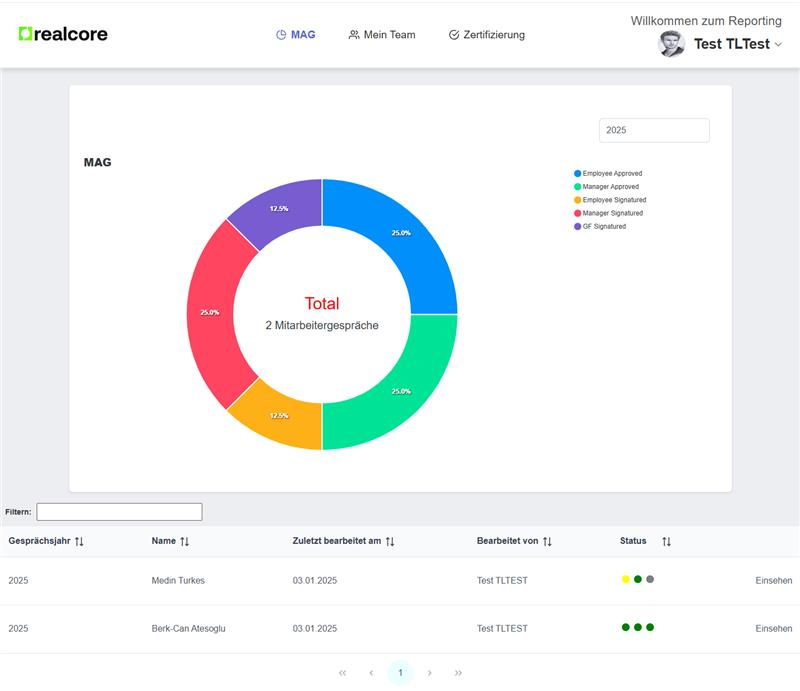
\includegraphics[angle=90, width=1.0\textwidth]{images/donutchart.jpg}
    \caption{Dashboard der Anwendung mit Donutchart und Übersicht über alle Mitarbeitendengespräche}
    \label{fig:dashboard}
\end{figure}


\begin{figure}[H]
    \centering
    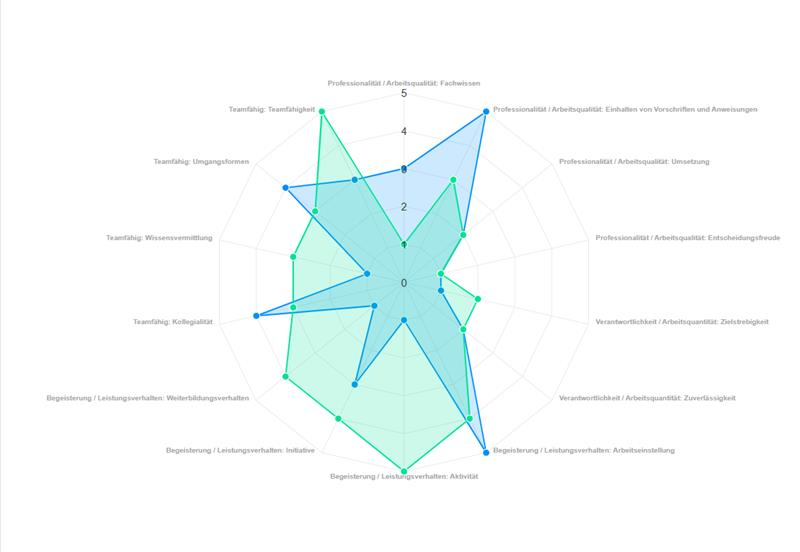
\includegraphics[angle=90, width=1.2\textwidth]{images/radarchart.jpg}
    \caption{Radarchart-Visualisierung der 1-5 Single Choice Antworten der Mitarbeitendengesprächsdaten}
    \label{fig:radar_chart}
\end{figure}

\begin{figure}[H]
    \centering
    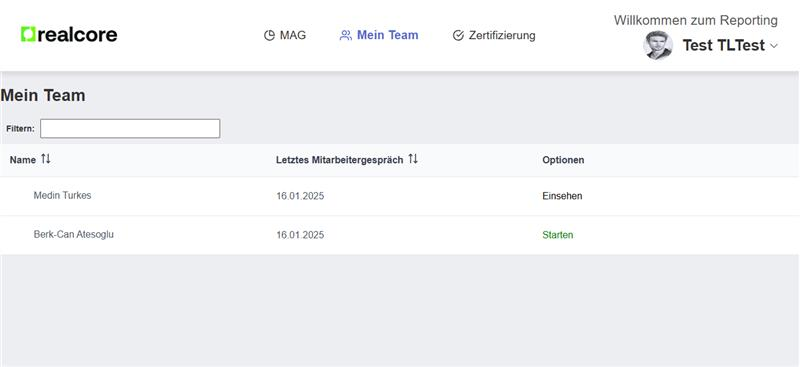
\includegraphics[width=1.2\textwidth]{images/meinteamview.jpg}
    \caption{Mein Team - Anzeige der Teammitglieder}
    \label{fig:data_entry}
\end{figure}

\begin{figure}[H]
    \centering
    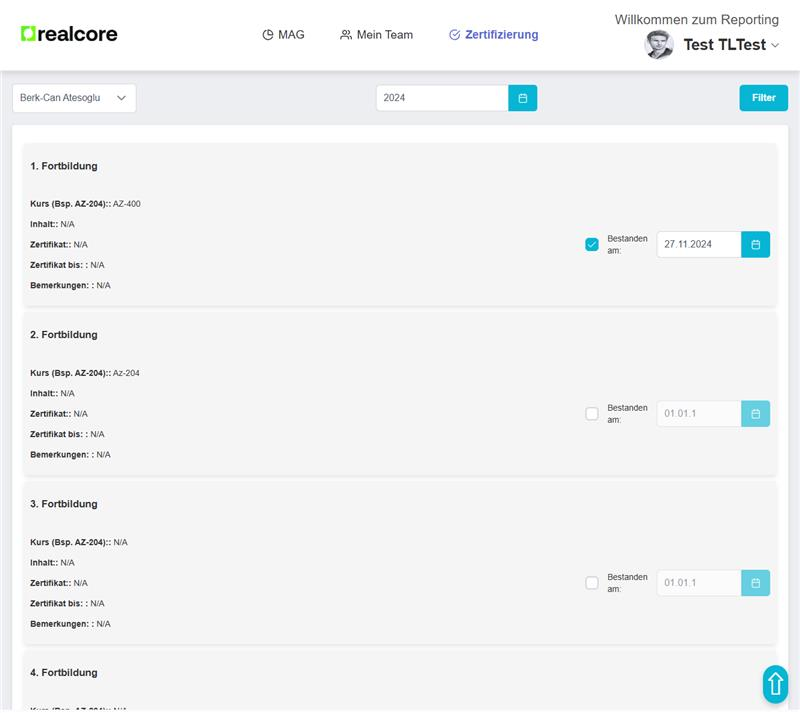
\includegraphics[width=1.2\textwidth]{images/zertifikatview.jpg}
    \caption{Zertifizierung - Anzeige von Mitarbeiterzertifizierungen}
    \label{fig:settings}
\end{figure}


\subsubsection*{Dockerfile für das Frontend}
Die Umsetzung des Frontends wurde durch die Nutzung von Docker als Containerisierungsplattform unterstützt, um eine konsistente Entwicklungs- und Produktionsumgebung zu gewährleisten. Das im Projekt verwendete Dockerfile basiert auf einem Multi-Stage-Build-Ansatz, der die Effizienz und Sicherheit der Anwendung optimiert. Im ersten Schritt wird die Anwendung mit Node.js gebaut, während im zweiten Schritt ein NGINX-Server verwendet wird, um die optimierten Dateien auszuliefern. Dieser Ansatz minimiert die Größe des finalen Containers und verbessert die Performance der Anwendung \cite{docker2020mastery, docker2019production}.

\begin{listing}[H]
\begin{minted}[linenos, frame=single, fontsize=\small]{dockerfile}
# Stage 0: Build the application
FROM node:16 as build-stage

WORKDIR /app

COPY package*.json /app/
RUN npm install --force

COPY vite.config.ts /app/
COPY vitest.config.ts /app/
COPY . /app/

RUN npm run build

# Stage 1: Serve the application using NGINX
FROM nginx:1.21
COPY --from=build-stage /app/dist/ /usr/share/nginx/html
\end{minted}
\caption{Dockerfile zur Containerisierung des Frontends}
\label{lst:dockerfile_frontend}
\end{listing}

In der ersten Build-Stage wird das Node.js-Image genutzt, das von der offiziellen Node.js-Docker-Bibliothek bereitgestellt wird \cite{node2021docker}. Hier werden die notwendigen Abhängigkeiten installiert und der Build-Prozess der Anwendung durchgeführt. Die zweite Stage verwendet ein NGINX-Image, das speziell für den Einsatz als Webserver optimiert ist \cite{nginx2021docker}. Der Multi-Stage-Ansatz bietet den Vorteil, dass lediglich die notwendigen Dateien für den Betrieb in die zweite Stage übernommen werden, wodurch die Größe des finalen Containers reduziert wird \cite{docker2020mastery}.

Die Wahl von Docker und Multi-Stage-Builds basiert auf der hohen Flexibilität und Effizienz dieser Technologie. Im Vergleich zu herkömmlichen Deployment-Ansätzen bietet Docker eine standardisierte Umgebung, die Fehler durch abweichende Konfigurationen zwischen Entwicklungs- und Produktionssystemen minimiert \cite{docker2019production}. Durch die Verwendung von offiziellen Docker-Images für Node.js und NGINX wird zudem sichergestellt, dass aktuelle Sicherheitsstandards eingehalten werden \cite{node2021docker, nginx2021docker}.



\subsection{Backend-Architektur}
Das Backend basiert auf einer mehrschichtigen Architektur, die eine klare Trennung von Verantwortlichkeiten gewährleistet. Diese Architektur stellt die Grundlage für eine effiziente und skalierbare Verarbeitung von Mitarbeitendengesprächsdaten dar.


\subsection{Projektstruktur und Paradigma des Backends}

Die Projektstruktur, wie in Abbildung~\ref{fig:backend_code_paradigm} dargestellt, basiert auf modernen Softwareentwicklungsprinzipien und wurde so gestaltet, dass eine klare Trennung der Verantwortlichkeiten gewährleistet ist. Dies trägt erheblich zur Wartbarkeit und Skalierbarkeit der Anwendung bei. Die zentrale Logik für die Verarbeitung von HTTP-Anfragen ist in der Controller-Schicht implementiert. Diese Schicht fungiert als Schnittstelle zwischen dem Frontend und den Backend-Diensten. Sie übernimmt das Routing von Anfragen, orchestriert die Kommunikation mit den anderen Schichten und sorgt für die konsistente Bearbeitung der Daten. Die Geschäftslogik ist in der Handler-Schicht ausgelagert. Diese Struktur entlastet die Controller von komplexen Prozessen und fördert die Modularität. Ein Handler führt notwendige Berechnungen, Validierungen oder Orchestrierungen durch, bevor die Ergebnisse zurück an den Controller gegeben werden \cite{fowler2002patterns}.

Die Datenzugriffsschicht ist im Repository-Ordner organisiert. Hier werden CRUD-Operationen mithilfe von Entity Framework Core realisiert. Diese Abstraktionsebene sorgt für einen konsistenten und wartbaren Zugriff auf die Datenbank. Die Datenstrukturen, die innerhalb des Systems verwendet werden, sind im Ordner \texttt{Models} definiert. Diese Modelle dienen als Bindeglied zwischen den einzelnen Schichten und sichern die Konsistenz der Daten. Ergänzend dazu werden im \texttt{Helper}-Ordner wiederverwendbare Funktionen und Werkzeuge zentralisiert, wie beispielsweise Logging- oder Utility-Funktionen \cite{efCoreDocs2023}.

Ein weiteres wichtiges Element ist der \texttt{Consumer}-Ordner, der die Logik zur Verarbeitung von Nachrichten aus asynchronen Kommunikationssystemen wie dem Azure Service Bus enthält. Diese Struktur ermöglicht die Umsetzung eines Publish-Subscribe-Musters, das die Skalierbarkeit und Entkopplung von Systemkomponenten sicherstellt \cite{azureServiceBus2024}.

Die Konfigurationen des Systems werden in der Datei \texttt{appsettings.json} verwaltet. Hier sind Verbindungszeichenfolgen zur Datenbank, API-Schlüssel und andere Umgebungsvariablen hinterlegt. Diese zentrale Verwaltung ermöglicht eine einfache Anpassung der Anwendung an verschiedene Umgebungen, beispielsweise Entwicklung, Test oder Produktion \cite{microsoftCloudDesignPatterns}.

Abbildung~\ref{fig:backend_code_paradigm} veranschaulicht diese Projektstruktur. Sie zeigt die logische Organisation der Dateien und Ordner und verdeutlicht, wie die Trennung der Verantwortlichkeiten die Zusammenarbeit im Team sowie die Skalierbarkeit und Wartbarkeit der Anwendung erleichtert.

\begin{figure}[H]
    \centering
    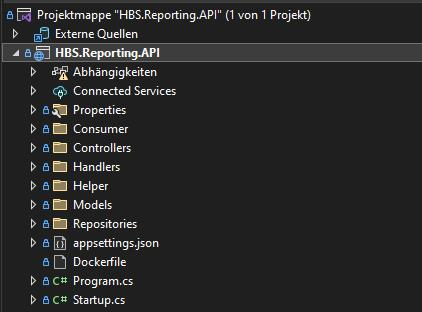
\includegraphics[width=0.6\textwidth, keepaspectratio]{images/backendparadigma.jpg}
    \caption{Projektstruktur des Backend-Paradigmas.}
    \label{fig:backend_code_paradigm}
\end{figure}

Diese strukturierte Herangehensweise bietet eine solide Grundlage für die Implementierung eines leistungsfähigen Backends. Durch die klare Trennung der Verantwortlichkeiten und die Verwendung bewährter Designprinzipien wird eine effiziente, skalierbare und wartungsfreundliche Architektur gewährleistet \cite{microsoftDotNetArchitecture}.




\subsection{Komponenten der Backend-Architektur}
Die Backend-Architektur folgt einer schichtbasierten Struktur, die eine klare Trennung von Verantwortlichkeiten ermöglicht. Diese modulare Architektur erleichtert die Wartbarkeit, Skalierbarkeit und Testbarkeit des Systems. Die Hauptkomponenten sind:

\begin{itemize}
     \item \textbf{Controller-Schicht:} Diese Schicht verarbeitet HTTP-Anfragen und leitet sie an entsprechende Services weiter. Alternativen wie GraphQL wurden geprüft, aber aufgrund der Einfachheit und Standardisierung fiel die Wahl auf RESTful APIs \cite{fielding2000rest}.

\begin{minted}[frame=single, fontsize=\small, linenos]{csharp}
using Microsoft.AspNetCore.Mvc;
using System.Threading.Tasks;

namespace HBS.Reporting.API.Controllers
{
    [ApiController]
    [Route("api/[controller]")]
    public class EmployeeAppraisalController : ControllerBase
    {
        private readonly IEmployeeAppraisalService _service;
        public EmployeeAppraisalController(IEmployeeAppraisalService service)
        {
            _service = service;
        }
        // GET: api/EmployeeAppraisal
        [HttpGet]
        public async Task<IActionResult> GetAll()
        {
            var appraisals = await _service.GetAllAppraisalsAsync();
            return Ok(appraisals);
        }
        // GET: api/EmployeeAppraisal/{id}
        [HttpGet("{id}")]
        public async Task<IActionResult> GetById(int id)
        {
            var appraisal = await _service.GetAppraisalByIdAsync(id);
            if (appraisal == null)
                return NotFound();
            return Ok(appraisal);
        }
        [HttpPost]
        public async Task<IActionResult> Create([FromBody] EmployeeAppraisalDto dto)
        {
            if (!ModelState.IsValid)
                return BadRequest(ModelState);

            var createdAppraisal = await _service.CreateAppraisalAsync(dto);
            return CreatedAtAction(nameof(GetById), new { id = createdAppraisal.Id }, createdAppraisal);
        }
        [HttpDelete("{id}")]
        public async Task<IActionResult> Delete(int id)
        {
            var isDeleted = await _service.DeleteAppraisalAsync(id);
            if (!isDeleted)
                return NotFound();
            return NoContent();
        }
    }
}
\end{minted}

Dieser Code stellt einen Beispiel-Controller für die Verwaltung von Mitarbeitendengesprächen bereit. Die \texttt{GetAll}-Methode ruft alle vorhandenen Datensätze ab, während \texttt{GetById} spezifische Einträge anzeigt. Mit \texttt{Create} können neue Einträge erstellt und über \texttt{Delete} wieder gelöscht werden. Alle Anfragen werden an die Service-Schicht delegiert, was die Trennung von Logik und Schnittstellen gewährleistet.

    \item \textbf{Service-Schicht:} Diese Schicht implementiert die Geschäftslogik und orchestriert zwischen Controllern und Repositories. Alternativansätze, wie eine direkte Einbindung der Logik in die Controller, wurden verworfen, da sie die Wartbarkeit reduzieren würden.
    \item \textbf{Repository-Schicht:} Diese Schicht abstrahiert die Datenbankzugriffe mithilfe von Entity Framework Core und sorgt für konsistente Operationen \cite{efCoreDocs2023}.
    \item \textbf{Middleware:} Hier werden zentrale Funktionen wie Authentifizierung und Fehlerbehandlung implementiert, was die Controllerschicht entlastet.
\end{itemize}

\subsection{API-Endpunkte}
Zur Interaktion mit den Daten des Systems wurden verschiedene API-Endpunkte implementiert. Tabelle \ref{table:http-methods} listet die wesentlichen HTTP-Methoden und URLs zur Manipulation von Ressourcen:

\begin{table}[H]
\caption{HTTP-Methoden und URLs zur Manipulation von Ressourcen}
\label{table:http-methods}
\raggedright
{\scriptsize Quelle: Eigene Darstellung} \\[0.3em]
\renewcommand{\arraystretch}{1.1}
\setlength{\tabcolsep}{1.8pt}
\begin{tabularx}{\textwidth}{>{\centering\arraybackslash}m{2cm}|>{\centering\arraybackslash}m{5.5cm}|>{\raggedright\arraybackslash}m{6.5cm}}
\hline
\textbf{HTTP-Methoden} & \textbf{URL /odata/v\{version\}} & \textbf{Beschreibung} \\\hline
GET & /employeeAppraisals/\{appraisalId\} & Lese ein einzelnes Mitarbeitergespräch anhand der eindeutigen ID. \\\hline
GET & /employeeAppraisals & Lese alle Mitarbeitergespräche zur Analyse und Berichterstellung. \\\hline
POST & /employeeAppraisals & Erstelle ein neues Mitarbeitergespräch und speichere es im System. \\\hline
GET & /employeeAppraisals/all & Lese alle verfügbaren Mitarbeitergespräche, einschließlich archivierter Daten. \\\hline
GET & /employeeAppraisals/last & Lese die zuletzt eingetragenen Mitarbeitergespräche. \\\hline
POST & /employeeAppraisals/CheckBox & Erstelle oder aktualisiere Checkbox-Daten für Mitarbeitergespräche. \\\hline
\end{tabularx}
\end{table}


\subsection{Datenbank SQL Queries}
Die Tabelle \texttt{EmployeeAppraisalData} bildet die Grundlage für die Speicherung von Informationen zu Mitarbeitenden und deren Bewertungen. Sie speichert essenzielle Daten wie Name, Jobtitel und Standort, die zur Analyse und Berichterstellung verwendet werden.

\subsubsection*{Erstellung der Tabelle}
Die Tabelle \texttt{EmployeeAppraisalData} wird mit folgendem SQL-Befehl erstellt:

\begin{figure}[H]
    \centering
    \caption{SQL-Befehl zur Erstellung der Tabelle \texttt{EmployeeAppraisalData}}
    \label{fig:create_table_query}
    \begin{minted}[frame=single, fontsize=\small, linenos]{sql}
CREATE TABLE [dbo].[EmployeeAppraisalData] (
    [Id]                   INT            NOT NULL,
    [MicrosoftId]          NVARCHAR (255) NULL,
    [GivenName]            NVARCHAR (255) NULL,
    [Surname]              NVARCHAR (255) NULL,
    [FJobTitleId]          INT            NULL,
    [CurrentJobTitleSince] DATETIME       NULL,
    [FOfficeLocationId]    INT            NULL,
    [CreatedAt]            DATETIME2 (7)  DEFAULT (getutcdate()) NOT NULL,
    [UpdatedAt]            DATETIME2 (7)  DEFAULT (getutcdate()) NOT NULL,
    PRIMARY KEY CLUSTERED ([Id] ASC),
    CONSTRAINT [FK_JobTitleId] FOREIGN KEY ([FJobTitleId]) REFERENCES [dbo].[JobTitle] ([Id]),
    CONSTRAINT [FK_OfficeLocationId] FOREIGN KEY ([FOfficeLocationId]) REFERENCES [dbo].[OfficeLocation] ([Id])
);
    \end{minted}
\end{figure}

Abbildung~\ref{fig:create_table_query} zeigt den SQL-Befehl zur Erstellung der Tabelle. Diese Struktur ermöglicht es, Daten wie die ID, den Namen und die Position eines Mitarbeitenden effizient zu speichern. Zusätzlich enthalten die Felder \texttt{CreatedAt} und \texttt{UpdatedAt} Zeitstempel für die Nachverfolgbarkeit von Änderungen.

\subsubsection*{Einfügen von Daten}
Datensätze werden mithilfe des folgenden SQL-Befehls in die Tabelle eingefügt:

\begin{figure}[H]
    \centering
    \caption{SQL-Befehl zum Einfügen eines Datensatzes in die Tabelle \texttt{EmployeeAppraisalData}}
    \label{fig:insert_query}
    \begin{minted}[frame=single, fontsize=\small, linenos]{sql}
INSERT INTO [dbo].[EmployeeAppraisalData] 
    ([Id], [MicrosoftId], [GivenName], [Surname], [FJobTitleId], [CurrentJobTitleSince], [FOfficeLocationId])
VALUES
    (1, 'microsoft123', 'John', 'Doe', 101, '2022-05-01', 201);
    \end{minted}
\end{figure}

Abbildung~\ref{fig:insert_query} demonstriert, wie ein neuer Datensatz mit spezifischen Informationen, wie etwa der ID \texttt{1} und dem Jobtitel, eingefügt wird. Fremdschlüssel wie \texttt{FJobTitleId} und \texttt{FOfficeLocationId} gewährleisten die Referenzierung zu den Tabellen \texttt{JobTitle} und \texttt{OfficeLocation}.

\subsubsection*{Abfrage von Daten}
Zum Abrufen von Daten aus der Tabelle kann der folgende SQL-Befehl genutzt werden:

\begin{figure}[H]
    \centering
    \caption{SQL-Befehl zur Abfrage von Daten aus \texttt{EmployeeAppraisalData}}
    \label{fig:select_query}
    \begin{minted}[frame=single, fontsize=\small, linenos]{sql}
SELECT 
    [Id], [GivenName], [Surname], [CurrentJobTitleSince], [FJobTitleId]
FROM 
    [dbo].[EmployeeAppraisalData]
WHERE 
    [FOfficeLocationId] = 201;
    \end{minted}
\end{figure}

Abbildung~\ref{fig:select_query} zeigt eine Abfrage, die alle Mitarbeitenden mit der Bürostandort-ID \texttt{201} aus der Tabelle \texttt{EmployeeAppraisalData} selektiert. Diese Daten können für die Erstellung von Berichten oder die Analyse von Trends verwendet werden.
Die Tabelle \texttt{EmployeeAppraisalData} bildet das zentrale Datenmodell zur Verwaltung von Mitarbeitendendaten. Die SQL-Befehle zur Erstellung, zum Einfügen und zum Abfragen von Daten zeigen, wie diese Struktur effektiv genutzt wird, um relevante Informationen zu speichern und zu analysieren. Die Kombination aus relationalem Modell und SQL-Abfragen stellt sicher, dass die Daten konsistent und leicht zugänglich sind.








\subsection{Fehleranalyse und Herausforderungen während der Implementierung}

Während der Implementierung traten verschiedene Herausforderungen auf, insbesondere bei der Integration von Datenvisualisierungen und der Kommunikation zwischen verschiedenen Systemkomponenten. Im Folgenden werden die zentralen Fehlerquellen und deren Lösungen erläutert.

\subsubsection*{Herausforderungen bei der Datenvisualisierung im Radarchart}

\item \textbf{Fehler 1: Datenintegration für Radarcharts}
Bei der Integration des Radarcharts ins Reporting-System traten Schwierigkeiten auf, die Daten aus den Mitarbeitendengesprächen sowohl für Mitarbeitende als auch für Manager korrekt darzustellen. Ursprünglich sollten die Single-Choice-Fragen visualisiert werden, um Unterschiede zwischen beiden Bewertungen leicht erkennbar zu machen. Die initiale Datenstruktur war jedoch nicht kompatibel mit den Anforderungen der Visualisierung, was zu Darstellungsfehlern führte.  
\textbf{Lösung:} Die Datenstruktur im Backend wurde angepasst, um die erforderlichen Daten vorzuverarbeiten und im gewünschten Format an das Frontend zu übermitteln.

\item \textbf{Fehler 2: Unübersichtliche Darstellung der Antworten}  
Die Darstellung der Antworten von Mitarbeitenden und Managern war unübersichtlich, da beide Bewertungen untereinander gelistet wurden. Dies erschwerte den direkten Vergleich und führte zu Verwirrung.  
\textbf{Lösung:} Die Darstellung wurde überarbeitet, sodass die Antworten von Mitarbeitenden und Managern nun nebeneinander angezeigt werden. Dies ermöglicht einen intuitiven Vergleich und unterstützt die Analyse von Unterschieden.

\subsubsection*{Herausforderungen mit Azure Service Bus}

\item \textbf{Fehler 3: Falsche Verbindungszeichenfolge (Connection String)}  
Beim Versuch, Nachrichten über den Azure Service Bus zu senden, trat ein Verbindungsfehler auf, da die Verbindungszeichenfolge nicht korrekt konfiguriert war. Dies führte zu Unterbrechungen in der Kommunikation zwischen Backend und Service Bus.  
\textbf{Lösung:} Die Verbindungszeichenfolge wurde in der Konfigurationsdatei (\texttt{appsettings.json}) korrigiert und Zugriffsrechte für den Service Bus wurden überprüft und angepasst.

\item \textbf{Fehler 4: Fehlende Nachrichtenfilterung bei Topic-Subscriptions}  
Nachrichten wurden an alle Konsumenten gesendet, auch wenn diese nicht relevant waren. Dies führte zu ineffizienten Verarbeitungsabläufen und hoher Serverlast.  
\textbf{Lösung:} SQL-basierte Filter wurden für die Topic-Subscriptions implementiert, um sicherzustellen, dass nur relevante Nachrichten an die entsprechenden Konsumenten weitergeleitet werden.

